
\section{Trees}
\begin{figure}
\center
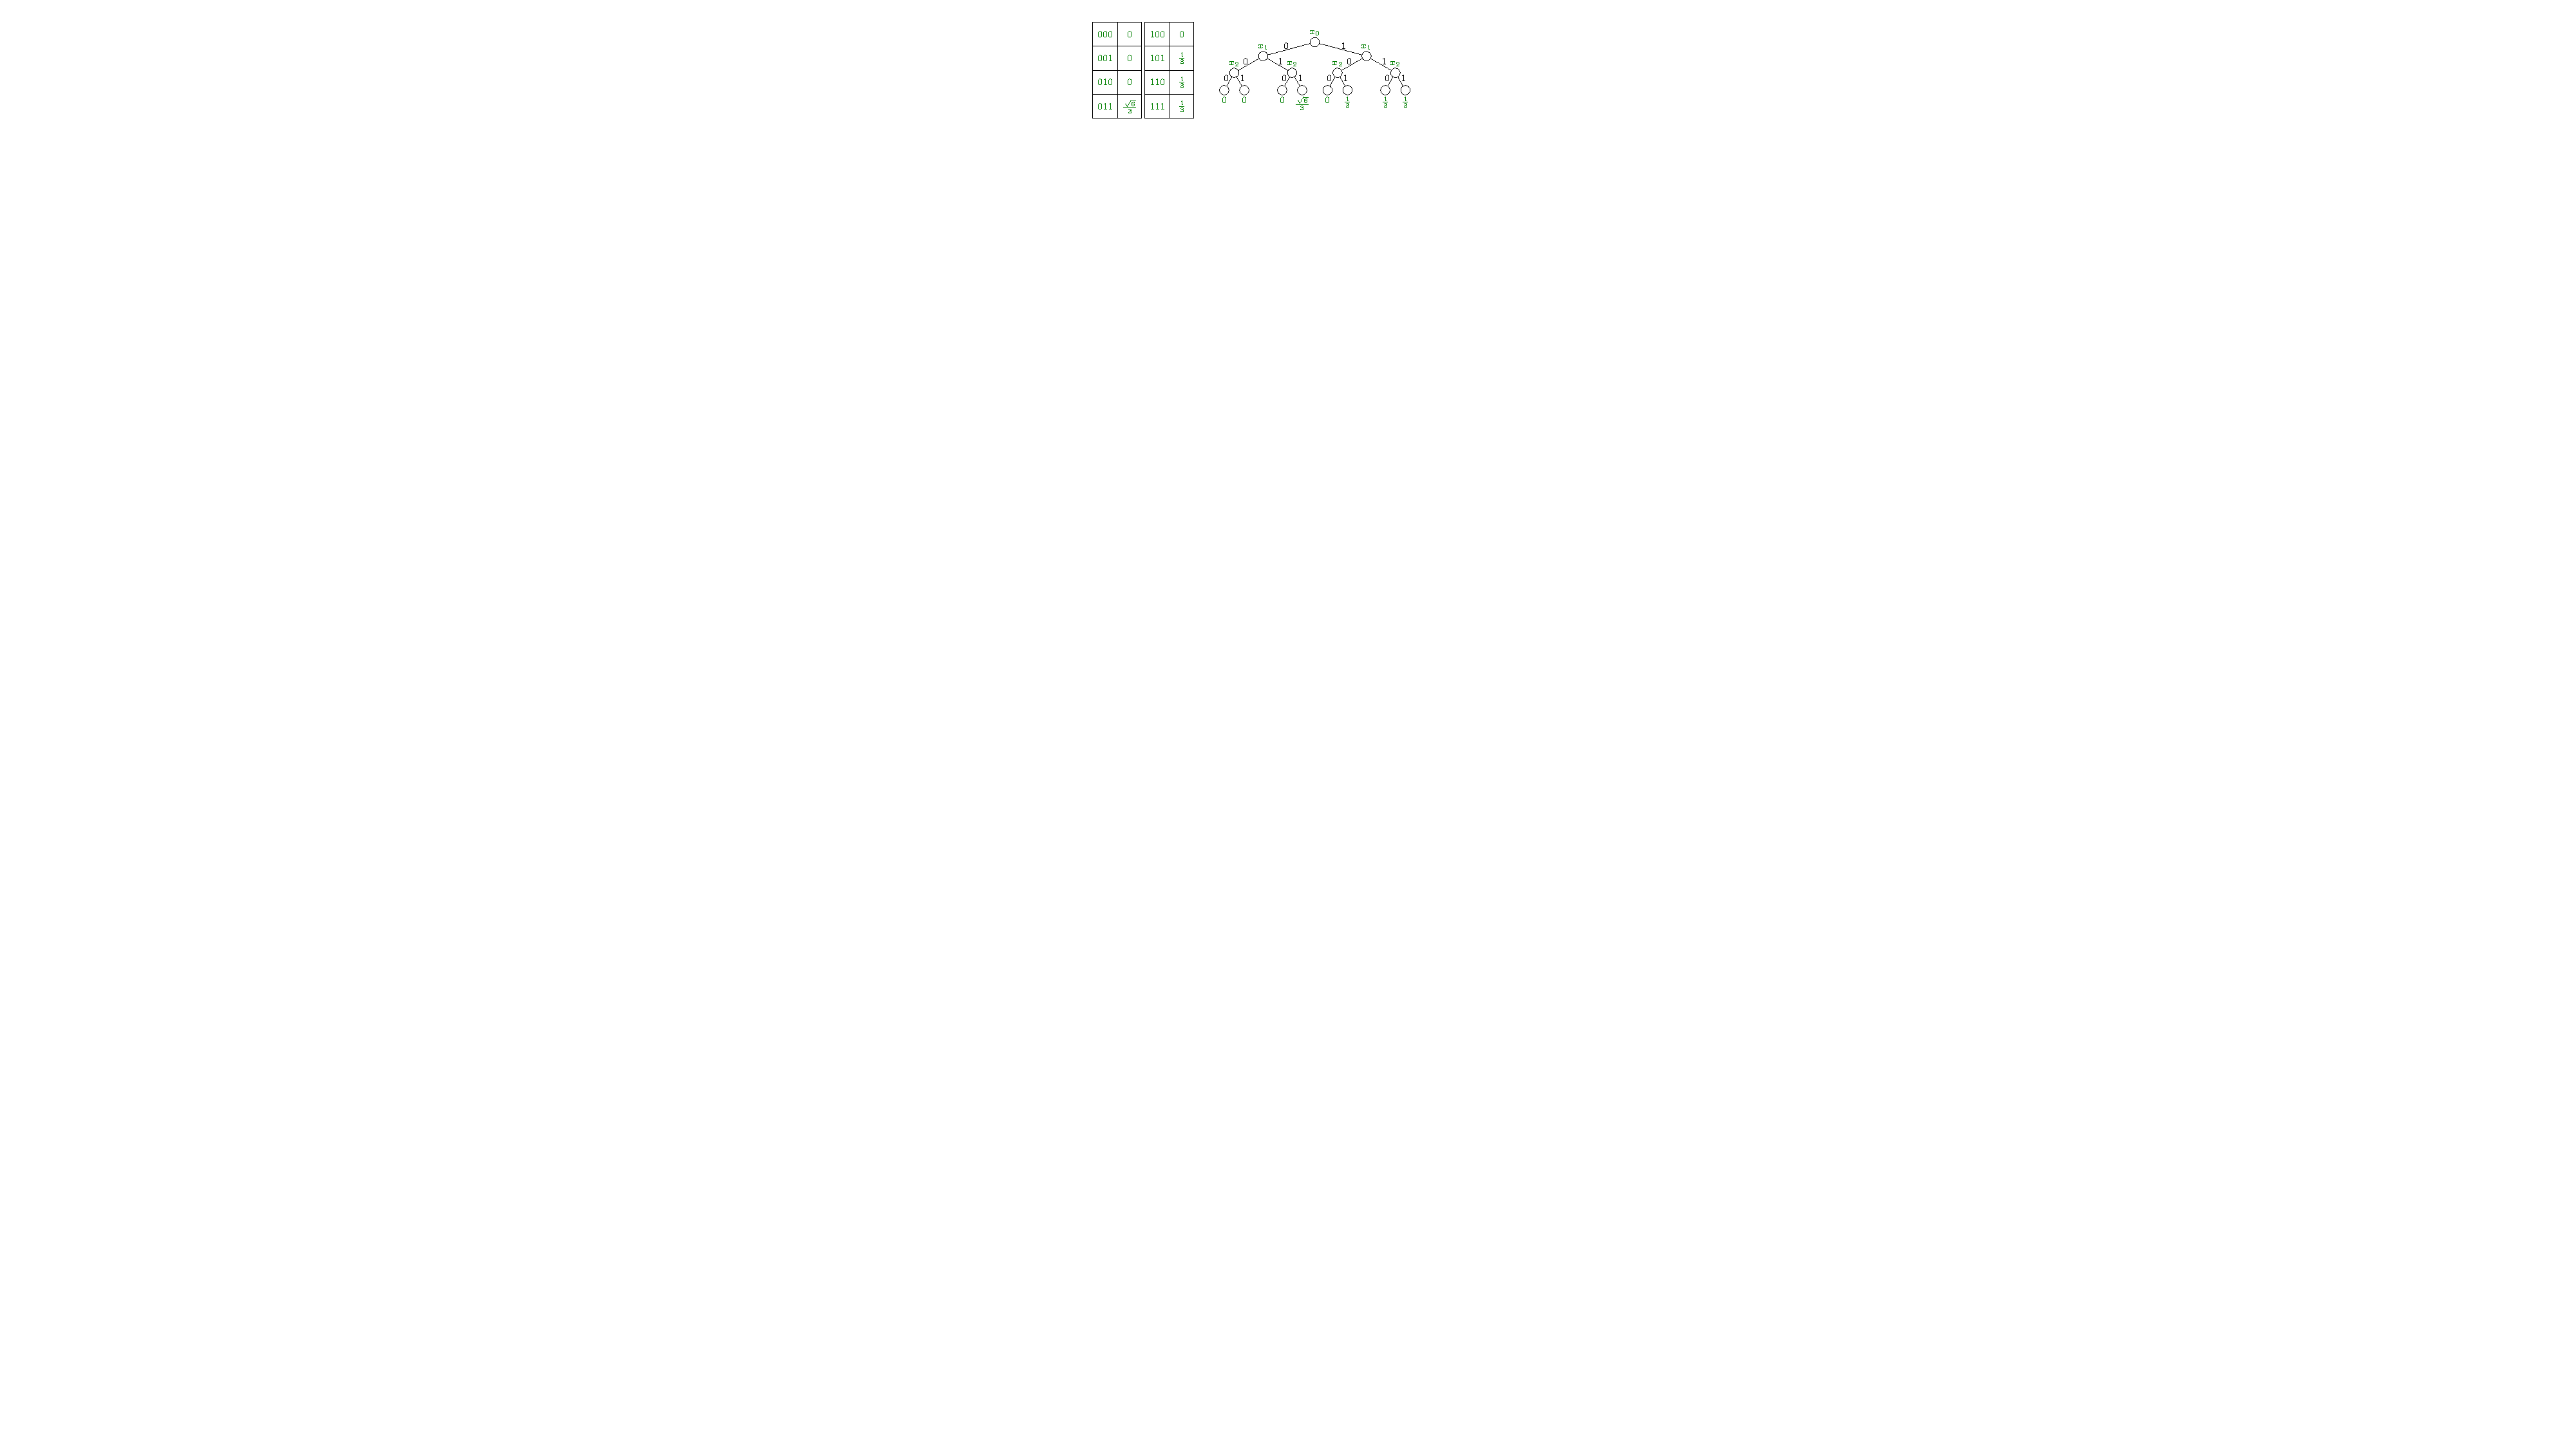
\includegraphics[]{Figures/Trees/Tree}
\caption{A quantum state with three qubits and its representation}
\label{qustate:tree:fig}
\end{figure}


\patodo{How about BDDs and classical tree automata?}


\begin{figure}
\center
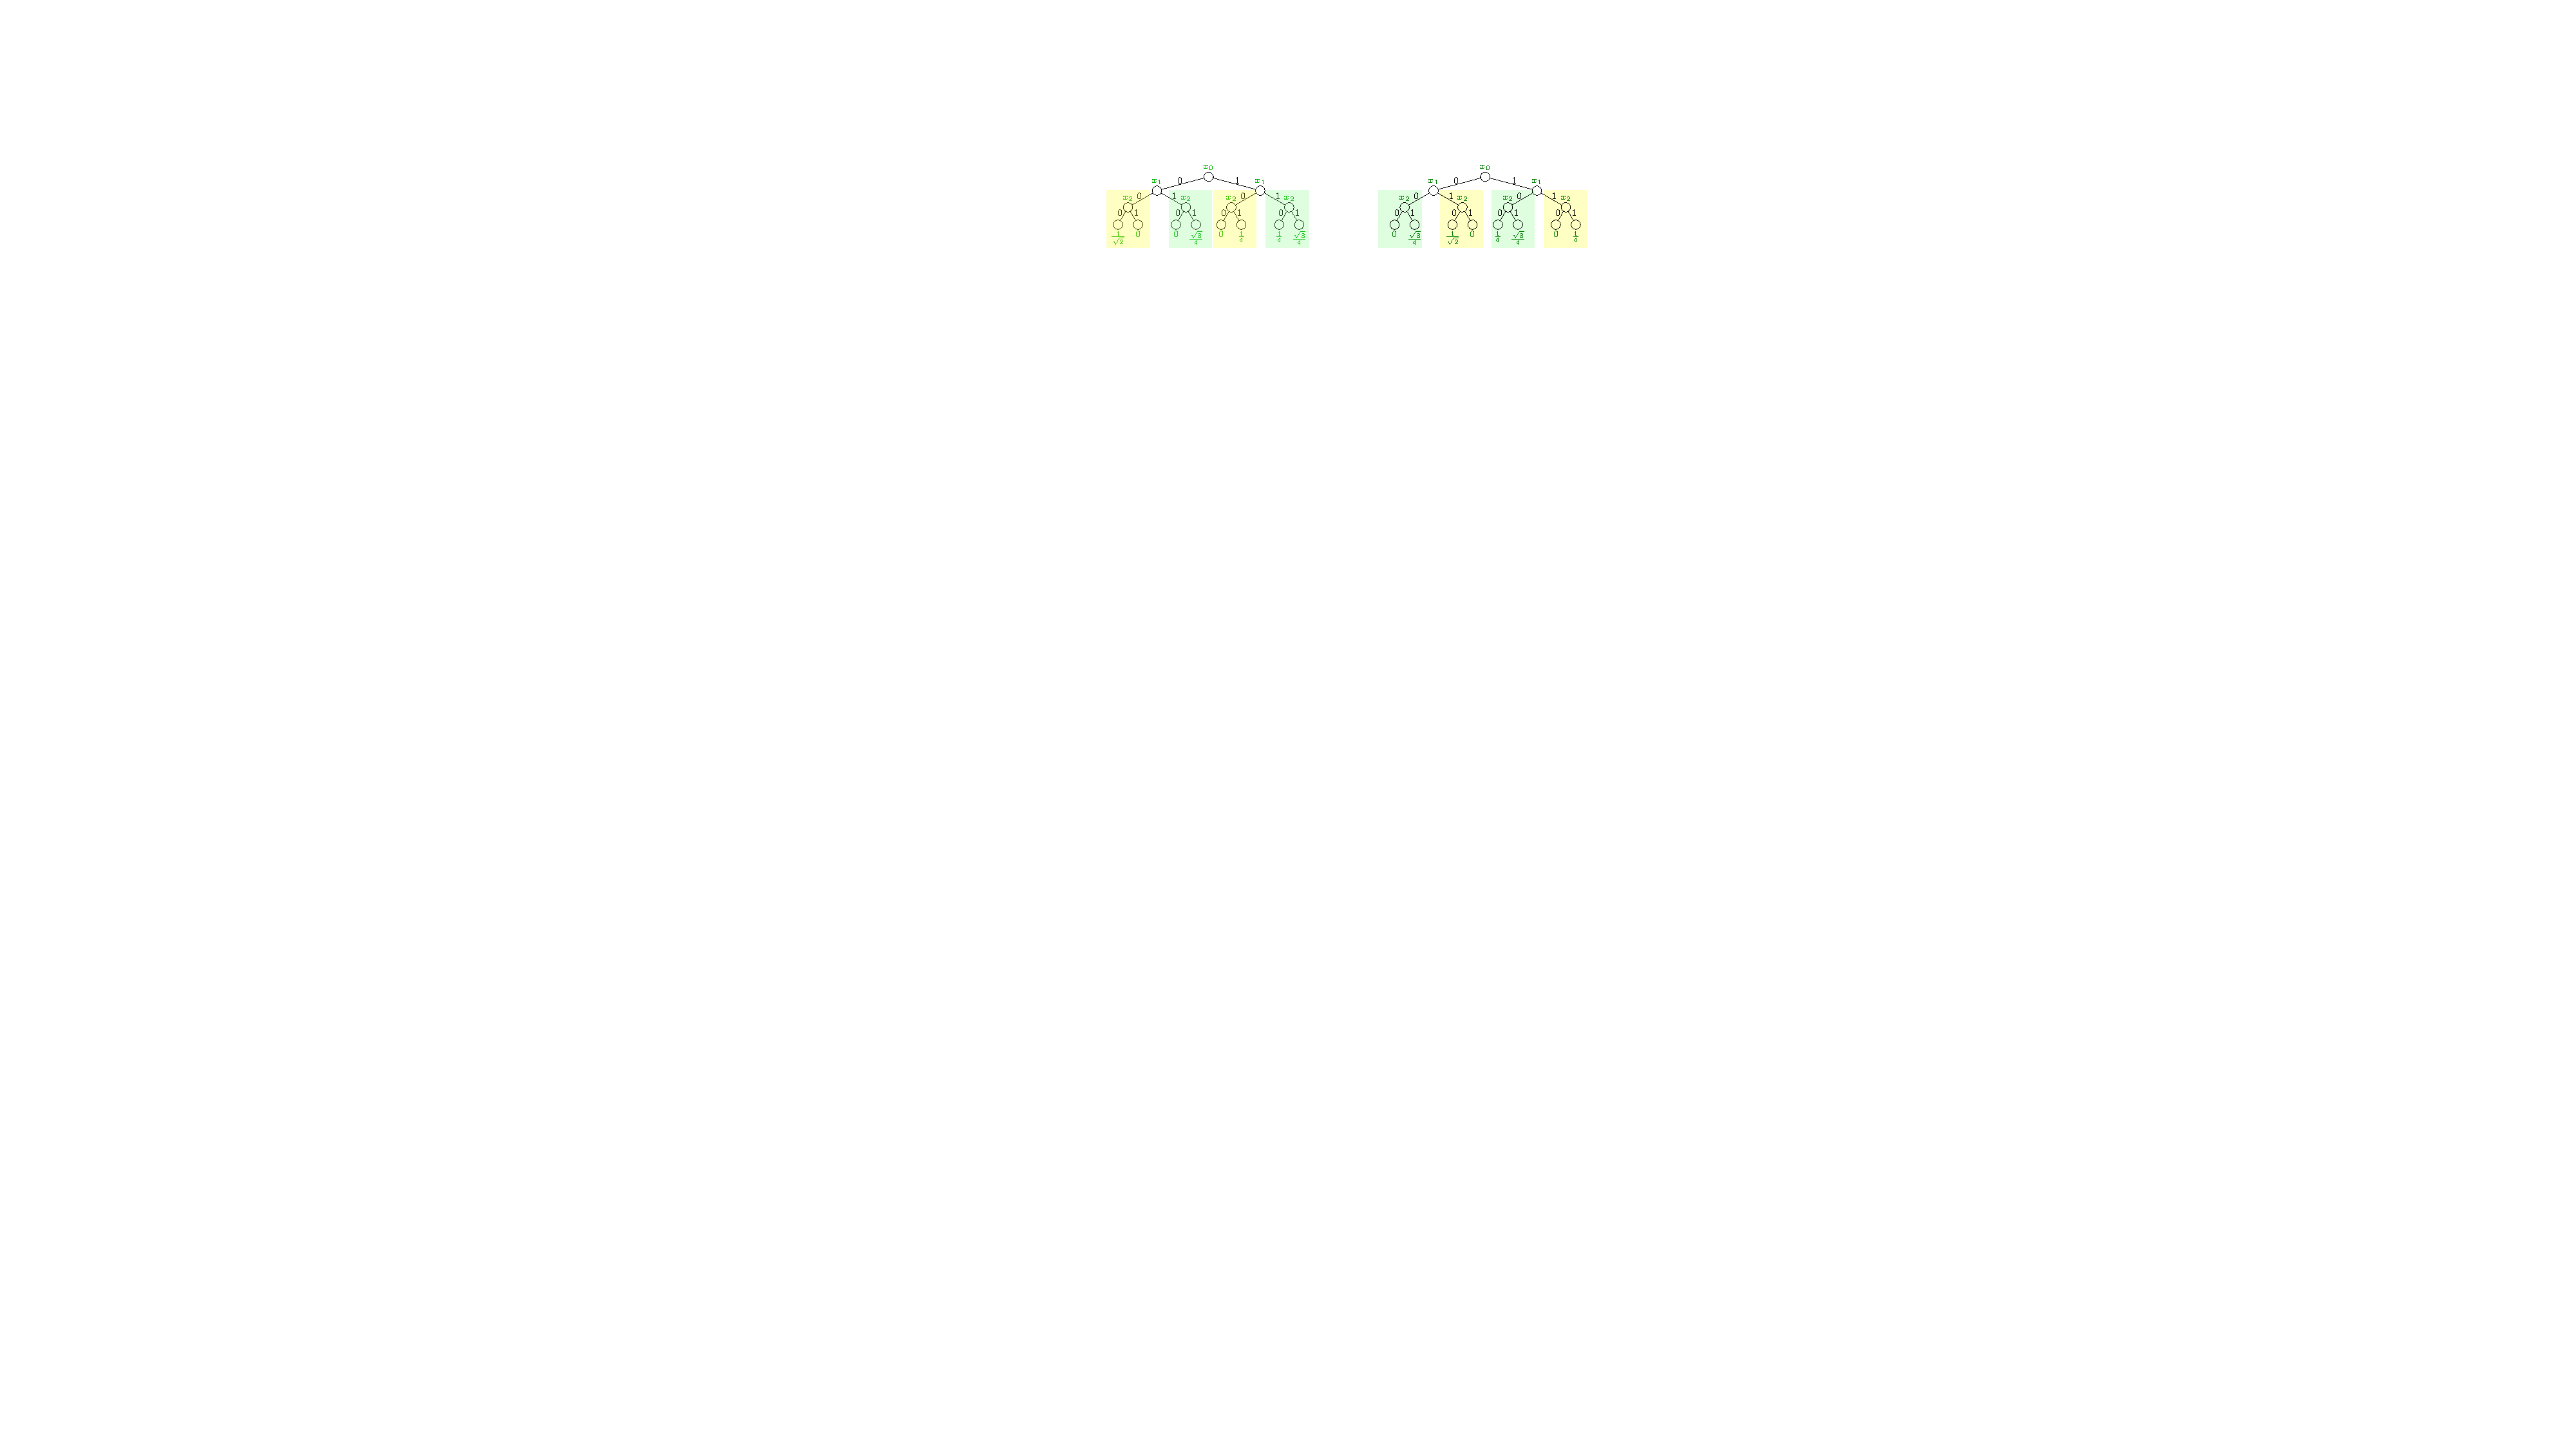
\includegraphics[]{Figures/Trees/ApplyNOT}
\caption{Applying the NOT gate to the second qubit.}
\label{apply:not:fig}
\end{figure}
%
In \ref{apply:not:fig}, we depict the result of applying the CNOT gate on the quantum state represented by the tree $\itree1$.
%
We obtain a new state represented, by the tree $\itree2$, where we swap the left- and righ-subtrres of each node at level $2$ of the tree.

\begin{figure}
\center
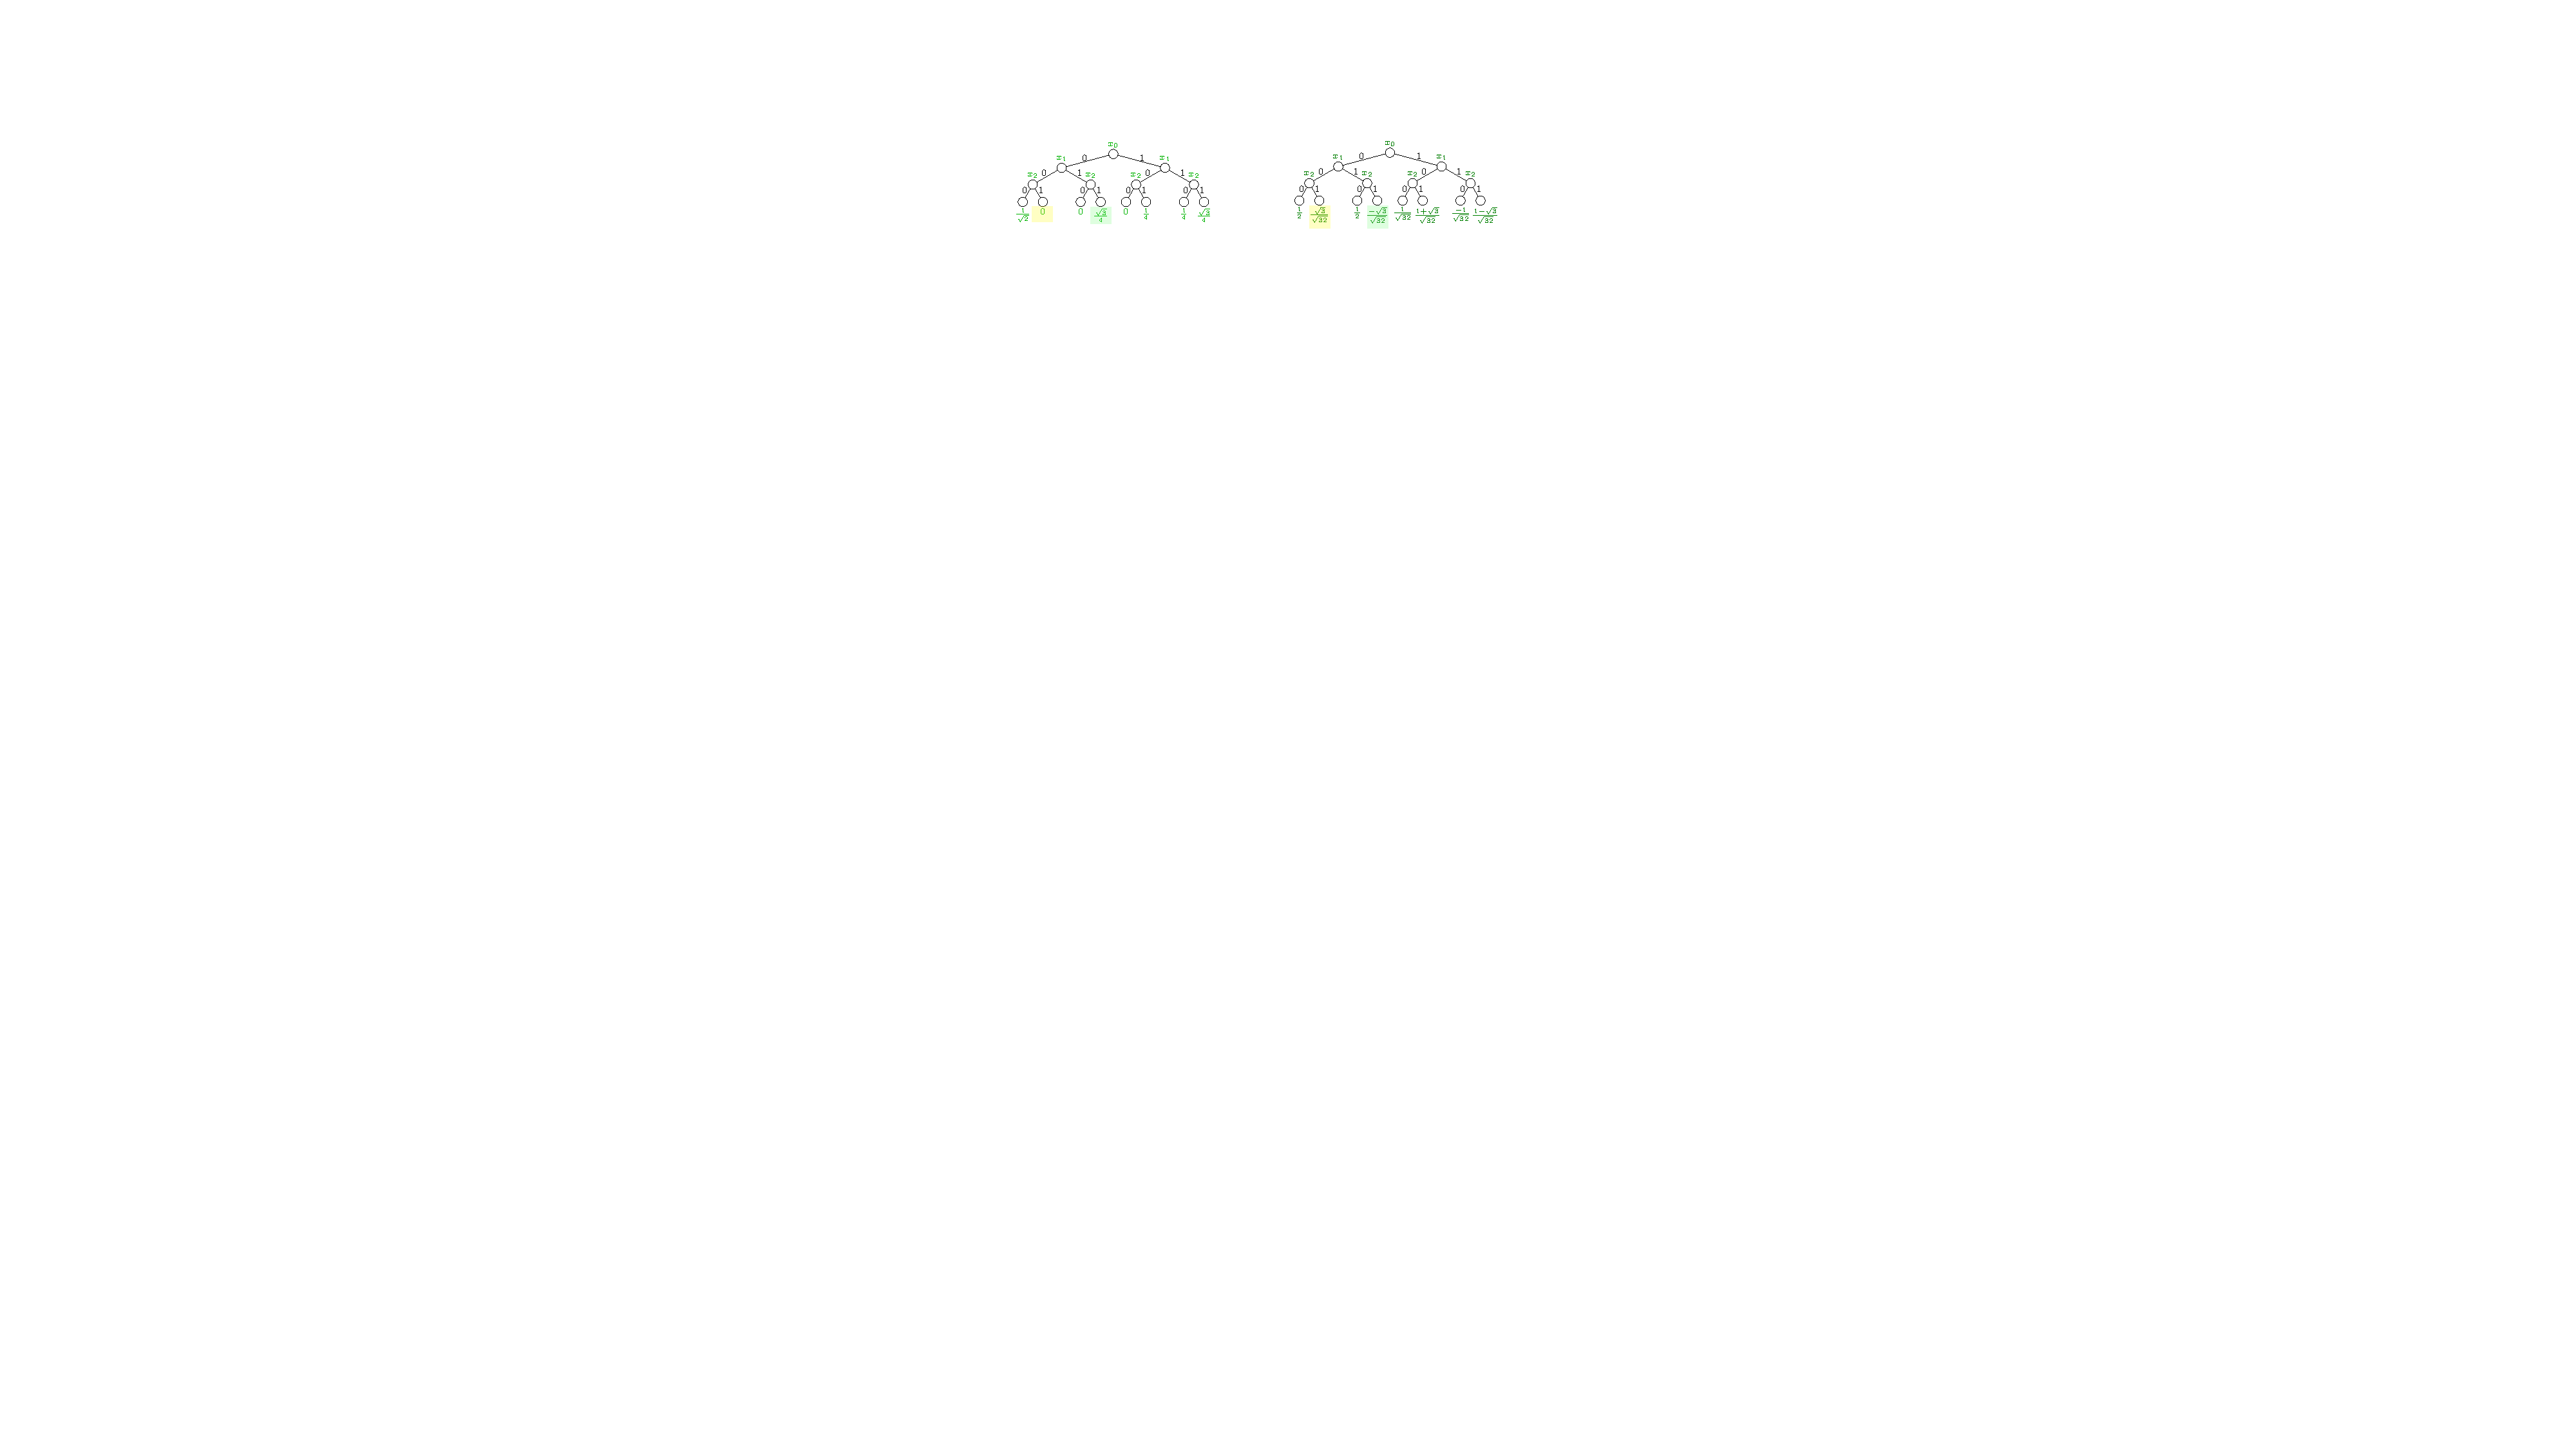
\includegraphics[]{Figures/Trees/ApplyH}
\caption{Applying the H gate to the second qubit.}
\label{apply:H:fig}
\end{figure}
